\chapter{Lateral particle probability fit parameters}
\label{app:lpp-fit-parameters}

\begin{figure}[H]
	\centering
    \rotatebox{90}{
        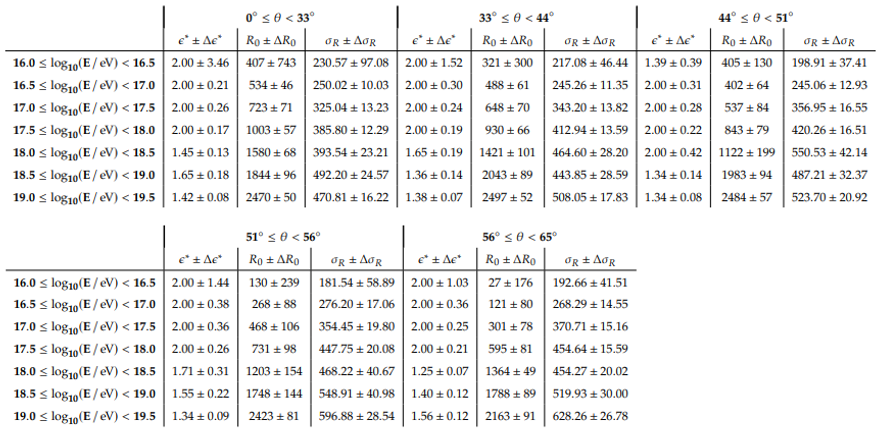
\includegraphics[width=0.7\paperheight]{./imgs/combined_LPP_params.png}
    }
	\caption{The best fit parameters $\epsilon^*$, $R_0$ [\SI{}{\meter}], and $\sigma_R$ [\SI{}{\per\meter}] for approximately vertical showers (left) and inclined
    showers (right).}
	\label{fig:fitfunction-comparison}
\end{figure}

% \footnotesize
% \begingroup
% \renewcommand{\arraystretch}{1.5}
% \begin{center}
%     \rotatebox{90}{
%     \begin{tabular}{c|c|c|c|c|c|c|c|c|c}
%         \multicolumn{1}{c|}{} & 
%         \multicolumn{3}{|c|}{$\mathbf{0^\circ \leq \theta < 33^\circ}$} &
%         \multicolumn{3}{|c|}{$\mathbf{33^\circ \leq \theta < 44^\circ}$} &
%         \multicolumn{3}{|c}{$\mathbf{44^\circ \leq \theta < 51^\circ}$} \\

%         \multicolumn{1}{c|}{} & $\epsilon^* \pm \Delta\epsilon^*$ & $R_0 \pm \Delta R_0$ & $\sigma_R \pm \Delta\sigma_R$ &
%         $\epsilon^* \pm \Delta\epsilon^*$ & $R_0 \pm \Delta R_0$ & $\sigma_R \pm \Delta\sigma_R$ &
%         $\epsilon^* \pm \Delta\epsilon^*$ & $R_0 \pm \Delta R_0$ & $\sigma_R \pm \Delta\sigma_R$ \\


%         \hline

%         $\mathbf{16.0 \leq \log_{10}(E\,/\,\mathrm{eV}) < 16.5}$ & $2.00 \pm 3.46$ & $407 \pm 743$ & $230.57 \pm 97.08$ & $2.00 \pm 1.52$ & $321 \pm 300$ & $217.08 \pm 46.44$ & $1.39 \pm 0.39$ & $405 \pm 130$ & $198.91 \pm 37.41$ \\
%         $\mathbf{16.5 \leq \log_{10}(E\,/\,\mathrm{eV}) < 17.0}$ & $2.00 \pm 0.21$ & $534 \pm 46$ & $250.02 \pm 10.03$ & $2.00 \pm 0.30$ & $488 \pm 61$ & $245.26 \pm 11.35$ & $2.00 \pm 0.31$ & $402 \pm 64$ & $245.06 \pm 12.93$ \\
%         $\mathbf{17.0 \leq \log_{10}(E\,/\,\mathrm{eV}) < 17.5}$ & $2.00 \pm 0.26$ & $723 \pm 71$ & $325.04 \pm 13.23$ & $2.00 \pm 0.24$ & $648 \pm 70$ & $343.20 \pm 13.82$ & $2.00 \pm 0.28$ & $537 \pm 84$ & $356.95 \pm 16.55$ \\
%         $\mathbf{17.5 \leq \log_{10}(E\,/\,\mathrm{eV}) < 18.0}$ & $2.00 \pm 0.17$ & $1003 \pm 57$ & $385.80 \pm 12.29$ & $2.00 \pm 0.19$ & $930 \pm 66$ & $412.94 \pm 13.59$ & $2.00 \pm 0.22$ & $843 \pm 79$ & $420.26 \pm 16.51$ \\
%         $\mathbf{18.0 \leq \log_{10}(E\,/\,\mathrm{eV}) < 18.5}$ & $1.45 \pm 0.13$ & $1580 \pm 68$ & $393.54 \pm 23.21$ & $1.65 \pm 0.19$ & $1421 \pm 101$ & $464.60 \pm 28.20$ & $2.00 \pm 0.42$ & $1122 \pm 199$ & $550.53 \pm 42.14$ \\
%         $\mathbf{18.5 \leq \log_{10}(E\,/\,\mathrm{eV}) < 19.0}$ & $1.65 \pm 0.18$ & $1844 \pm 96$ & $492.20 \pm 24.57$ & $1.36 \pm 0.14$ & $2043 \pm 89$ & $443.85 \pm 28.59$ & $1.34 \pm 0.14$ & $1983 \pm 94$ & $487.21 \pm 32.37$ \\
%         $\mathbf{19.0 \leq \log_{10}(E\,/\,\mathrm{eV}) < 19.5}$ & $1.42 \pm 0.08$ & $2470 \pm 50$ & $470.81 \pm 16.22$ & $1.38 \pm 0.07$ & $2497 \pm 52$ & $508.05 \pm 17.83$ & $1.34 \pm 0.08$ & $2484 \pm 57$ & $523.70 \pm 20.92$ \\
%     \end{tabular}
%     }
% \end{center}
% \endgroup
% \normalsize

% \footnotesize
% \begingroup
% \renewcommand{\arraystretch}{1.5}
% \begin{center}
%     \rotatebox{90}{
%     \begin{tabular}{c|c|c|c|c|c|c}
%         \multicolumn{1}{c|}{} & 
%         \multicolumn{3}{|c|}{$\mathbf{51^\circ \leq \theta < 56^\circ}$} &
%         \multicolumn{3}{|c}{$\mathbf{56^\circ \leq \theta < 65^\circ}$} \\

%         \multicolumn{1}{c|}{} & $\epsilon^* \pm \Delta\epsilon^*$ & $R_0 \pm \Delta R_0$ & $\sigma_R \pm \Delta\sigma_R$ &
%         $\epsilon^* \pm \Delta\epsilon^*$ & $R_0 \pm \Delta R_0$ & $\sigma_R \pm \Delta\sigma_R$ \\


%         \hline

%         $\mathbf{16.0 \leq \log_{10}(E\,/\,\mathrm{eV}) < 16.5}$ & $2.00 \pm 1.44$ & $130 \pm 239$ & $181.54 \pm 58.89$ & $2.00 \pm 1.03$ & $27 \pm 176$ & $192.66 \pm 41.51$ \\
%         $\mathbf{16.5 \leq \log_{10}(E\,/\,\mathrm{eV}) < 17.0}$ & $2.00 \pm 0.38$ & $268 \pm 88$ & $276.20 \pm 17.06$ & $2.00 \pm 0.36$ & $121 \pm 80$ & $268.29 \pm 14.55$ \\
%         $\mathbf{17.0 \leq \log_{10}(E\,/\,\mathrm{eV}) < 17.5}$ & $2.00 \pm 0.36$ & $468 \pm 106$ & $354.45 \pm 19.80$ & $2.00 \pm 0.25$ & $301 \pm 78$ & $370.71 \pm 15.16$ \\
%         $\mathbf{17.5 \leq \log_{10}(E\,/\,\mathrm{eV}) < 18.0}$ & $2.00 \pm 0.26$ & $731 \pm 98$ & $447.75 \pm 20.08$ & $2.00 \pm 0.21$ & $595 \pm 81$ & $454.64 \pm 15.59$ \\
%         $\mathbf{18.0 \leq \log_{10}(E\,/\,\mathrm{eV}) < 18.5}$ & $1.71 \pm 0.31$ & $1203 \pm 154$ & $468.22 \pm 40.67$ & $1.25 \pm 0.07$ & $1364 \pm 49$ & $454.27 \pm 20.02$ \\
%         $\mathbf{18.5 \leq \log_{10}(E\,/\,\mathrm{eV}) < 19.0}$ & $1.55 \pm 0.22$ & $1748 \pm 144$ & $548.91 \pm 40.98$ & $1.40 \pm 0.12$ & $1788 \pm 89$ & $519.93 \pm 30.00$ \\
%         $\mathbf{19.0 \leq \log_{10}(E\,/\,\mathrm{eV}) < 19.5}$ & $1.34 \pm 0.09$ & $2423 \pm 81$ & $596.88 \pm 28.54$ & $1.56 \pm 0.12$ & $2163 \pm 91$ & $628.26 \pm 26.78$ \\

%     \end{tabular}
%     }
% \end{center}
% \endgroup
% \normalsize